%\frameT{Outline}{
%  \begin{enumerate}
%    {\transparent{0.2} \item The languages of PLP-trees and LP-trees}
%    \item Learning preference models in case of PLP-trees
%    {\transparent{0.2} \item Reasoning with preferences:
%      \begin{itemize}
%        \item Computing winners and ``strong" candidates when votes are LP-trees
%        \item Application in trip planning
%      \end{itemize}}
%    {\transparent{0.2} \item Future research directions}
%  \end{enumerate}
%}
\frameT{Outline}{
  \begin{enumerate}
    {\transparent{0.2} \item Modeling qualitative preferences:
    \begin{itemize}
      \item Preference trees (P-trees)
      \item Partial lexicographic preference trees (PLP-trees)
    \end{itemize}}
    \item Learning PLP-trees and PLP-forests
    {\transparent{0.2} \item Aggregating LP-trees
    \item Future research directions}
  \end{enumerate}
}

%\frameT{The Cars Domain}{
%  \begin{enumerate}
%    \item \tbf{BodyType}(B): \{mvan, sedan, sport, suv\}.
%    \item \tbf{Capacity}(C): \{2, 5, 7m\}.
%    \item \tbf{Color}(O): \{black, blue, gray, red, white\}.
%    \item \tbf{LuggageSize}(L): \{big, med, small\}.
%    \item \tbf{Make}(M): \{bmw, ford, honda, vw\}.
%    \item \tbf{Price}(P): \{low, med, high, vhigh\}.
%    \item \tbf{Safety}(S): \{low, med, high\}.
%  \end{enumerate}
%}

\frameT{Learning PLP-trees}{
	\begin{block}{Consistent Learning (\tsc{ConsLearn})}
		Given an example set $\cE$, decide 
		whether there exists a PLP-tree $T$ (of a particular type) such that $T$ 
		is consistent with $\cE$.
	\end{block}
	\vspace{-0.3cm}

  \begin{figure}[ht]
     \small
    \centering
    \begin{subfigure}[b]{0.95\textwidth}
      \centering
      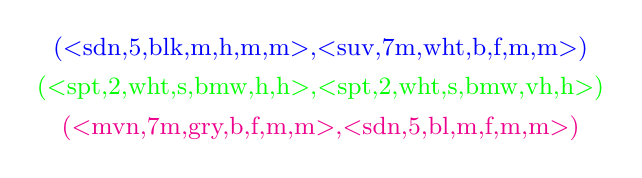
\begin{tikzpicture}[->,>=stealth,node distance=0.5cm,main node/.style={rectangle,font=\small}]
        \node[main node] (1)              {\textcolor{blue}{($<$sdn,5,blk,m,h,m,m$>$,$<$suv,7m,wht,b,f,m,m$>$)}}; 
        \node[main node] (2) [below of=1] {\textcolor{green}{($<$spt,2,wht,s,bmw,h,h$>$,$<$spt,2,wht,s,bmw,vh,h$>$)}};
        \node[main node] (3) [below of=2] {\textcolor{magenta}{($<$mvn,7m,gry,b,f,m,m$>$,$<$sdn,5,bl,m,f,m,m$>$)}};
      \end{tikzpicture}
      %\caption{Examples}
    \end{subfigure}\\ \vspace{0.5cm}
    \begin{subfigure}[b]{0.95\textwidth}
    	\centering
      \begin{tikzpicture}[->,>=stealth',
        level 1/.style={sibling distance=2cm, level distance=33pt},
        level 2/.style={sibling distance=0.7cm, level distance=27pt}
      ]

        \node[main node,inner sep=2pt] (1) {P};
        \node[rectangle,draw,inner sep=2pt] at (1.2,0) {\textcolor{green}{$m \!\!>\!\! h\!\!>\!\! l\!\!>\!\! vh$}};

        \node[main node,inner sep=2pt] (2) [below of=1] {M};
        \node[rectangle,draw,inner sep=2pt] at (1.52,-1) {\textcolor{blue}{$h \!\!>\!\! vw\!\!>\!\! f\!\!>\!\! bmw$}};

        \node[main node,inner sep=2pt] (3) [below of=2] {B};
        \node[rectangle,draw,inner sep=2pt] at (1.8,-2) {\textcolor{magenta}{$mvn\!\! >\!\! suv\!\! >\!\! sdn\!\! >\!\! spt$}};

        \path[every node/.style={font=\sffamily\small}]
          (1) edge (2)
          (2) edge (3);
      \end{tikzpicture}
      \caption*{UIUP tree}
    \end{subfigure}
  \end{figure}
}

\frameT{Learning PLP-trees}{
	\begin{block}{Small Learning (\tsc{SmallLearn})}
		Given an example set $\cE$
		and a positive integer $l$ ($l \leq |\cE|$), decide whether there 
		exists a PLP-tree $T$ (of a particular type) such that $T$ is consistent 
		with $\cE$ and $|T| \leq l$.
	\end{block}
	\vspace{-0.3cm}

  \begin{figure}[ht]
     \small
    \centering
    \begin{subfigure}[b]{0.95\textwidth}
      \centering
      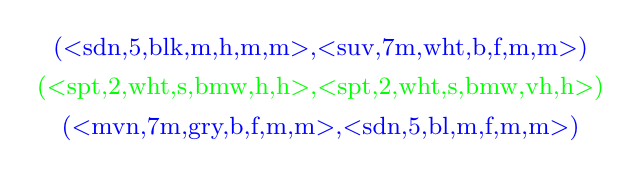
\begin{tikzpicture}[->,>=stealth,node distance=0.5cm,main node/.style={rectangle,font=\small}]
        \node[main node] (1)              {\textcolor{blue}{($<$sdn,5,blk,m,h,m,m$>$,$<$suv,7m,wht,b,f,m,m$>$)}}; 
        \node[main node] (2) [below of=1] {\textcolor{green}{($<$spt,2,wht,s,bmw,h,h$>$,$<$spt,2,wht,s,bmw,vh,h$>$)}};
        \node[main node] (3) [below of=2] {\textcolor{blue}{($<$mvn,7m,gry,b,f,m,m$>$,$<$sdn,5,bl,m,f,m,m$>$)}};
      \end{tikzpicture}
      %\caption{Examples}
    \end{subfigure}\\ \vspace{0.5cm}
    \begin{subfigure}[b]{0.95\textwidth}
    	\centering
      \begin{tikzpicture}[->,>=stealth',
        level 1/.style={sibling distance=2cm, level distance=33pt},
        level 2/.style={sibling distance=0.7cm, level distance=27pt}
      ]

        \node[main node,inner sep=2pt] (1) {B};
        \node[rectangle,draw,inner sep=2pt] at (1.8,0) {\textcolor{blue}{$mvn\!\! >\!\! sdn\!\! >\!\! suv\!\! >\!\! spt$}};

        \node[main node,inner sep=2pt] (2) [below of=1] {P};
        \node[rectangle,draw,inner sep=2pt] at (1.2,-1) {\textcolor{green}{$m \!\!>\!\! h\!\!>\!\! l\!\!>\!\! vh$}};

        \path[every node/.style={font=\sffamily\small}]
          (1) edge (2);
      \end{tikzpicture}
      \caption*{UIUP tree}
    \end{subfigure}
  \end{figure}
}

\frameT{Learning PLP-trees}{
	\begin{block}{Maixmal Learning (\tsc{MaxLearn})}
		Given an example set $\cE$ and a 
		positive integer $k$ ($k \leq m$), decide whether there exists a PLP-tree 
		$T$ (of a particular type) such that $T$ satisfies at least $k$ examples 
		in $\cE$.
	\end{block}
	\vspace{-0.3cm}

  \begin{figure}[ht]
     \small
    \centering
    \begin{subfigure}[b]{0.95\textwidth}
      \centering
      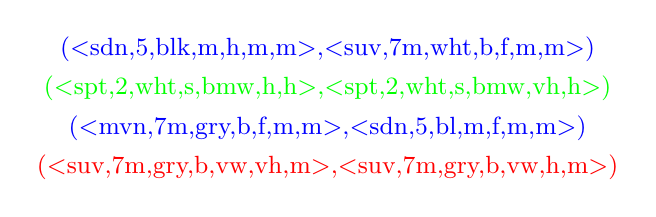
\begin{tikzpicture}[->,>=stealth,node distance=0.5cm,main node/.style={rectangle,font=\small}]
        \node[main node] (1)              {\textcolor{blue}{($<$sdn,5,blk,m,h,m,m$>$,$<$suv,7m,wht,b,f,m,m$>$)}}; 
        \node[main node] (2) [below of=1] {\textcolor{green}{($<$spt,2,wht,s,bmw,h,h$>$,$<$spt,2,wht,s,bmw,vh,h$>$)}};
        \node[main node] (3) [below of=2] {\textcolor{blue}{($<$mvn,7m,gry,b,f,m,m$>$,$<$sdn,5,bl,m,f,m,m$>$)}};
        \node[main node] (4) [below of=3] {\textcolor{red}{($<$suv,7m,gry,b,vw,vh,m$>$,$<$suv,7m,gry,b,vw,h,m$>$)}};
      \end{tikzpicture}
      %\caption{Examples}
    \end{subfigure}\\ \vspace{0.5cm}
    \begin{subfigure}[b]{0.95\textwidth}
    	\centering
      \begin{tikzpicture}[->,>=stealth',
        level 1/.style={sibling distance=2cm, level distance=33pt},
        level 2/.style={sibling distance=0.7cm, level distance=27pt}
      ]

        \node[main node,inner sep=2pt] (1) {B};
        \node[rectangle,draw,inner sep=2pt] at (1.8,0) {\textcolor{blue}{$mvn\!\! >\!\! sdn\!\! >\!\! suv\!\! >\!\! spt$}};

        \node[main node,inner sep=2pt] (2) [below of=1] {P};
        \node[rectangle,draw,inner sep=2pt] at (1.2,-1) {\textcolor{green}{$m \!\!>\!\! h\!\!>\!\! l\!\!>\!\! vh$}};

        \path[every node/.style={font=\sffamily\small}]
          (1) edge (2);
      \end{tikzpicture}
      \caption*{UIUP tree}
    \end{subfigure}
  \end{figure}
}

%\frameT{Learning PLP-trees}{
%	\begin{block}{Consistent Learning (\tsc{ConsLearn})}
%		Given an example set $\cE$, decide 
%		whether there exists a PLP-tree $T$ (of a particular type) such that $T$ 
%		is consistent with $\cE$.
%	\end{block}
%	\vspace{-0.3cm}
%
%  \begin{figure}[ht]
%     \small
%    \centering
%    \begin{subfigure}[b]{0.95\textwidth}
%      \centering
%      \begin{tikzpicture}[->,>=stealth,node distance=0.5cm,main node/.style={rectangle,font=\small}]
%        \node[main node] (1)              {\textcolor{blue}{($<$sdn,5,blk,m,h,m,m$>$,$<$suv,7m,wht,b,f,m,m$>$)}}; 
%        \node[main node] (2) [below of=1] {\textcolor{green}{($<$spt,2,wht,s,bmw,h,h$>$,$<$spt,2,wht,s,bmw,vh,h$>$)}};
%        \node[main node] (3) [below of=2] {\textcolor{blue}{($<$mvn,7m,gry,b,f,m,m$>$,$<$sdn,5,bl,m,f,m,m$>$)}};
%        \node[main node] (4) [below of=3] {\textcolor{red}{($<$suv,7m,gry,b,vw,vh,m$>$,$<$suv,7m,gry,b,vw,h,m$>$)}};
%      \end{tikzpicture}
%      %\caption{Examples}
%    \end{subfigure}\\ \vspace{0.5cm}
%    \begin{subfigure}[b]{0.95\textwidth}
%    	\centering
%      \begin{tikzpicture}[->,>=stealth',
%        level 1/.style={sibling distance=2cm, level distance=33pt},
%        level 2/.style={sibling distance=0.7cm, level distance=27pt}
%      ]
%
%        \node[main node,inner sep=2pt] (1) {B};
%        \node[rectangle,draw,inner sep=2pt] at (1.8,0) {\textcolor{blue}{$mvn\!\! >\!\! sdn\!\! >\!\! suv\!\! >\!\! spt$}};
%
%        \node[main node,inner sep=2pt] (2) [below of=1] {P};
%        \node[rectangle split, rectangle split parts=4, draw,inner sep=2pt,font=\sffamily\small] at (1.6,-1.5)
%            {
%              \textcolor{green}{$spt\!:m \!\!>\!\! h\!\!>\!\! l\!\!>\!\! vh$}
%              \nodepart{second}
%              \textcolor{red}{$suv\!:vh \!\!>\!\! h\!\!>\!\! m\!\!>\!\! l$}
%              \nodepart{third}
%              $mvn\!:\!m \!\!>\!\! h\!\!>\!\! l\!\!>\!\! vh$
%              \nodepart{fourth}
%              $sdn\!:\!m \!\!>\!\! h\!\!>\!\! l\!\!>\!\! vh$
%            };
%
%        \path[every node/.style={font=\sffamily\small}]
%          (1) edge (2);
%      \end{tikzpicture}
%      \caption*{UICP tree}
%    \end{subfigure}
%  \end{figure}
%}

%\frameT{Learning PLP-trees}{
%	\begin{block}{Consistent Learning (\tsc{ConsLearn})}
%		Given an example set $\cE$, decide 
%		whether there exists a PLP-tree $T$ (of a particular type) such that $T$ 
%		is consistent with $\cE$.
%	\end{block}
%
%	\begin{block}{Small Learning (\tsc{SmallLearn})}
%		Given an example set $\cE$
%		and a positive integer $l$ ($l \leq |\cE|$), decide whether there 
%		exists a PLP-tree $T$ (of a particular type) such that $T$ is consistent 
%		with $\cE$ and $|T| \leq l$.
%	\end{block}
%
%	\begin{block}{Maixmal Learning (\tsc{MaxLearn})}
%		Given an example set $\cE$ and a 
%		positive integer $k$ ($k \leq m$), decide whether there exists a PLP-tree 
%		$T$ (of a particular type) such that $T$ satisfies at least $k$ examples 
%		in $\cE$.
%	\end{block}
%}

%\frameT{Computational Complexity}{
%  \begin{enumerate}
%    \item $P$, $\NP$, $\coNP$: We typically believe that $P \subset \NP$ and $P \subset \coNP$.
%    %\item $\coNP$: problems whose complements are in $\NP$.
%    \item $\deltap{2}$: $P^\NP$, $\sigmap{2}$: $\NP^\NP$, and $\pip{2}$: $\coNP^\NP$.
%    \item $C$-complete: hardest decision problems in class $C$.
%    %\item A decision problem $L$ is $C$-hard if $L' \leq_p L$ for every $L'$ in class $C$.
%    %\item A decision problem $L$ is $C$-complete if $L$ is in class $C$ and $L$ is $C$-hard.
%  \end{enumerate}
%
%  \vspace{-0.3cm}
%
%  \begin{figure}[ht!]
%    \centering
%      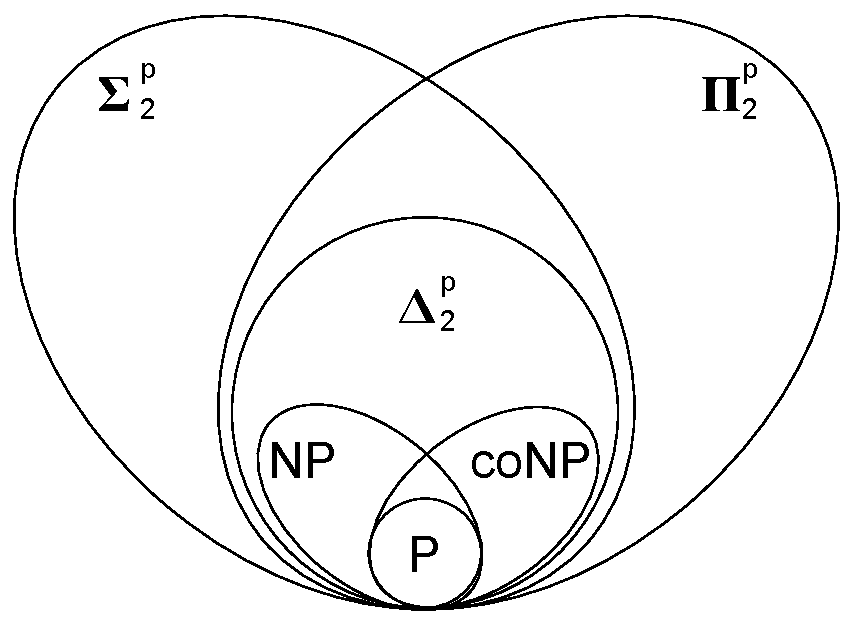
\includegraphics[width=0.5\textwidth]{figs/Preliminary/comp_diagram.pdf}
%    \caption{Computational complexity diagram}
%  \end{figure}
%}

\frameT{Complexity Results on PLP-trees} {
  \begin{figure}[!ht]
    \centering
    \begin{subfigure}[b]{0.45\textwidth}
      \centering
      \begin{tabular}[0.45\textwidth]{ | c | c | c | }
        \hline
           & UP & CP \\
        \hline
        UI & P & NP\\
        \hline
        CI & NPC\footnotemark & P  \\
        \hline
      \end{tabular}
      \caption{\tsc{ConsLearn}}
    \end{subfigure}
      \footnotetext{\scriptsize Booth et al., \tit{Learning Conditionally Lexicographic
            Preference Relations}, 2010.}
    \begin{subfigure}[b]{0.45\textwidth}
      \centering
      \begin{tabular}[0.45\textwidth]{ | c | c | c | }
        \hline
           & UP & CP \\
        \hline
        UI & NPC & NPC \\
        \hline
        CI & NPC & NPC \\
        \hline
      \end{tabular}
      \caption{\tsc{SmallLearn}}
    \end{subfigure} \\
    \begin{subfigure}[b]{0.45\textwidth}
      \centering
      \begin{tabular}[0.45\textwidth]{ | c | c | c | }
        \hline
           & UP & CP \\
        \hline
        UI & NPC\footnotemark & NPC \\
        \hline
        CI & NPC & NPC \\
        \hline
      \end{tabular}
      \caption{\tsc{MaxLearn}}
    \end{subfigure}
    \caption{Complexity results for learning PLP-trees}
  \end{figure}
  \footnotetext{\scriptsize Schmitt and Martignon, \tit{On the Complexity of
            Learning Lexicographic Strategies}, 2006.}
}

\frameT{Experimentation}{
  \begin{figure}[ht!]
    \centering
      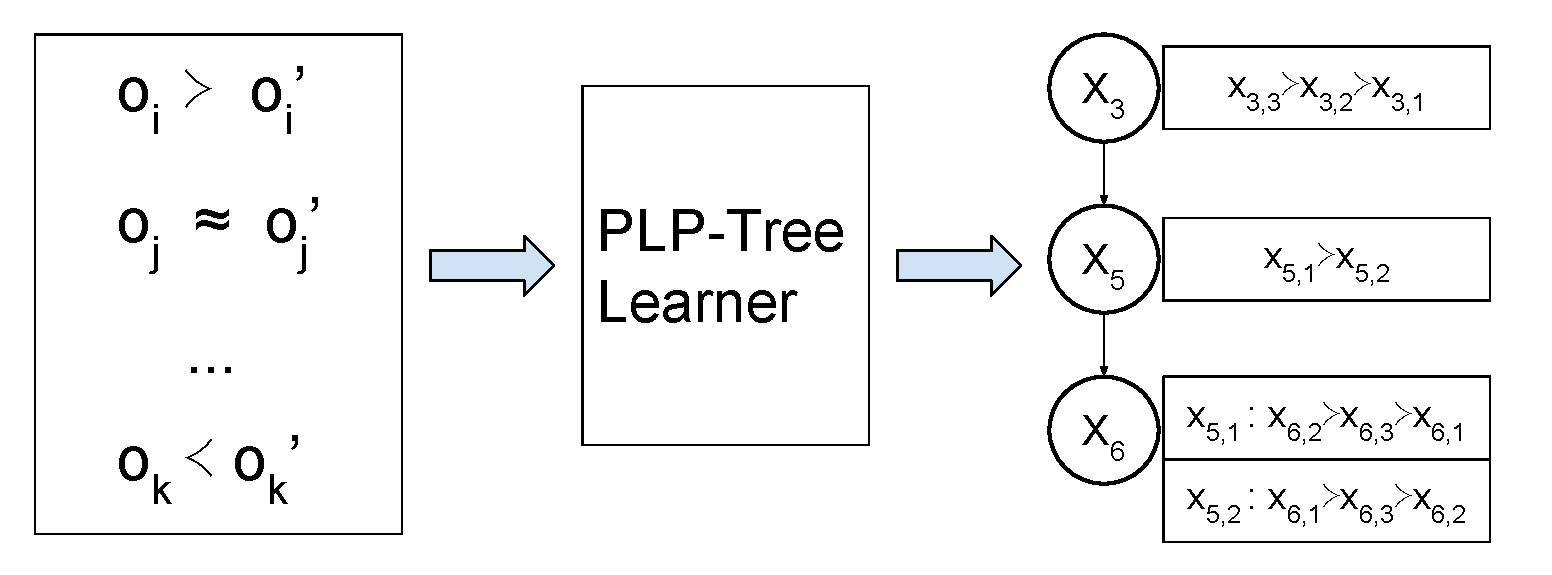
\includegraphics[width=0.9\textwidth]{figs/PrefLearnResults/LearningPLPT.pdf}
    \caption{PLP-tree learning system}
  \end{figure}

}

\frameT{Datasets}{
	\begin{figure}
		\centering
		\small
		\begin{tabular}{ |c||c|c|c|c| } 
			\hline
			Dataset                 & $p$  & $|\cX|$ & $|\cE^\succ|$ & $|\cE^\approx|$ \\
			\hline \hline
			BreastCancerWisconsin   & 9    & 270 & 9,009 & 27,306 \\ \hline
			CarEvaluation           & 6    & 1,728 & 682,721 & 809,407\\ \hline
			CreditApproval          & 10   & 520 & 66,079 & 68,861 \\ \hline
			GermanCredit            & 10   & 914 & 172,368 & 244,873 \\ \hline
			Ionosphere              & 10   & 118 & 3,472 & 3,431 \\	\hline
			MammographicMass        & 5    & 62 & 792 & 1,099 \\	\hline
			Mushroom                & 10   & 184 & 8,448 & 8,388 \\	\hline
			Nursery                 & 8    & 1,266 & 548,064 & 252,681 \\	\hline
			SPECTHeart              & 10   & 115 & 3,196 & 3,359 \\	\hline
			TicTacToe               & 9    & 958 & 207,832 & 250,571 \\ \hline
			Vehicle                 & 10   & 455 & 76,713 & 26,572 \\ \hline
			Wine                    & 10   & 177 & 10,322 & 5,254 \\
			\hline
		\end{tabular}
		\caption{Preference Learning Library\footnotemark}
	\end{figure}

	\footnotetext{\tiny \url{http://www.cs.uky.edu/~liu/preflearnlib.php}}
}

%\frameT{PLP-Trees To Learn}{
%  \begin{figure}[ht!]
%    \centering
%      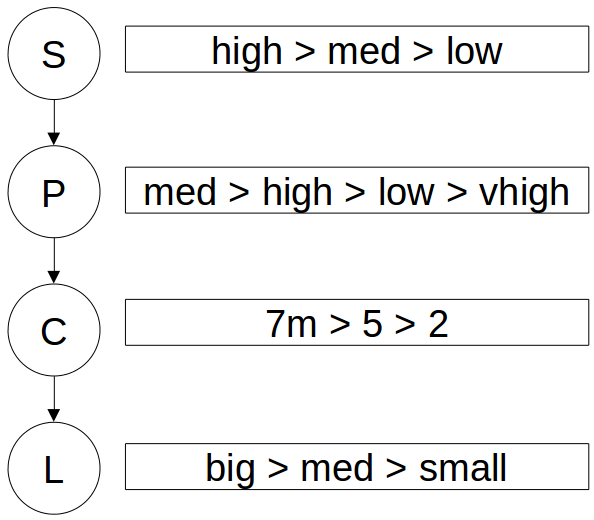
\includegraphics[width=0.4\textwidth]{figs/Cars/uiuptree.png}
%    \caption{Unconditional Importance \& Unconditional Preference (UIUP)}
%  \end{figure}
%}
%
%\frameT{PLP-Trees To Learn}{
%  \begin{figure}[ht!]
%    \centering
%      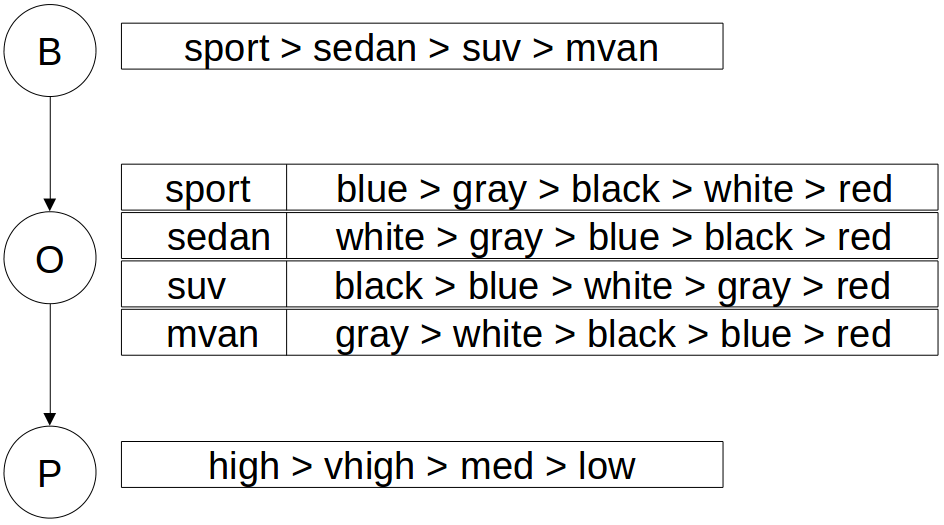
\includegraphics[width=0.65\textwidth]{figs/Cars/uicptree.png}
%    \caption{UICP with at most 1 parent (UICP-1)}
%  \end{figure}
%}
%
%\frameT{PLP-Trees To Learn}{
%  \begin{figure}[ht!]
%    \centering
%      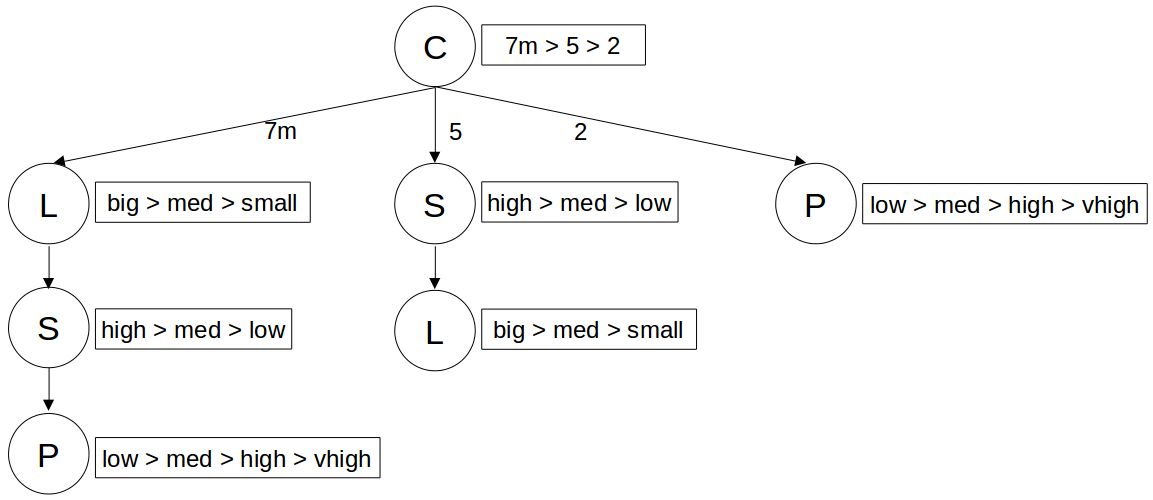
\includegraphics[width=0.9\textwidth]{figs/Cars/ciuptree.png}
%    \caption{CIUP with 1 split at the root (CIUP-1)}
%  \end{figure}
%}
%
%\frameT{PLP-Trees To Learn}{
%  \begin{figure}[ht!]
%    \centering
%      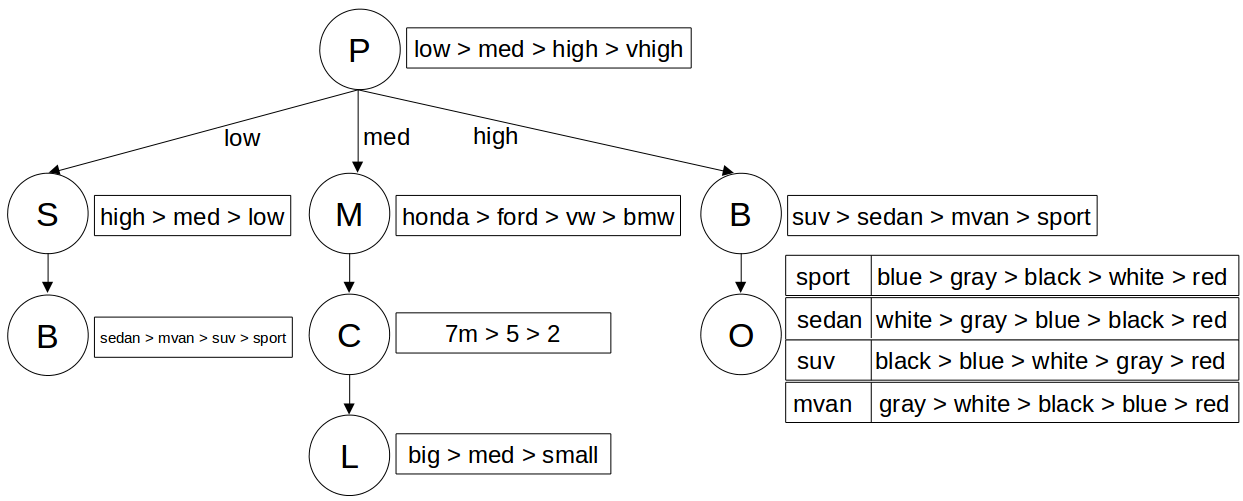
\includegraphics[width=0.9\textwidth]{figs/Cars/cicptree.png}
%    \caption{Simple CICP (SCICP)}
%  \end{figure}
%}

\frameT{Experimental Results: Best-Agreement vs. Greedy}
{
	\begin{table}
	  \centering
		\small
	  \begin{tabular}{ |c||c|c| }
	    \hline
	    Dataset               & BA-UIUP           & G-UIUP \\
	    \hline \hline                               
	    BreastCancerWisconsin & \tbf{88.4}        & 88.2     \\ \hline
	    CarEvaluation         & \tbf{84.8}        & 83.6     \\ \hline
	    CreditApproval        & \tbf{91.1}        & 89.3     \\ \hline
	    GermanCredit          & \tbf{72.2}        & 72.2     \\ \hline
	    Ionosphere            & \tc{\tbf{87.0}}   & 79.6     \\ \hline
	    MammographicMass      & \tbf{87.5}        & 86.8     \\ \hline
	    Mushroom              & \tc{\tbf{84.8}}   & 70.3     \\ \hline
	    Nursery               & \tbf{91.8}        & 91.7     \\ \hline
	    SPECTHeart            & \tbf{93.2}        & 92.6     \\ \hline
	    TicTacToe             & \tbf{72.1}        & 71.9     \\ \hline
	    Vehicle               & \tbf{76.8}        & 76.6     \\ \hline
	    Wine                  & \tbf{96.0}        & 95.5     \\ \hline
	  \end{tabular}
	  \caption{Accuracy (percentage of correctly handled testing examples)
						 for UIUP PLP-trees learned using the best-agreement and
						 the greedy methods on the learning 
						 data (250 of $\cE^\succ$)}
	  \label{tbl:trees1}
	\end{table}
}

\frameT{Experimental Results: Best-Agreement vs. Greedy}
{
  \begin{figure}
    \centering
    \begin{subfigure}[b]{0.3\textwidth}
      \centering
      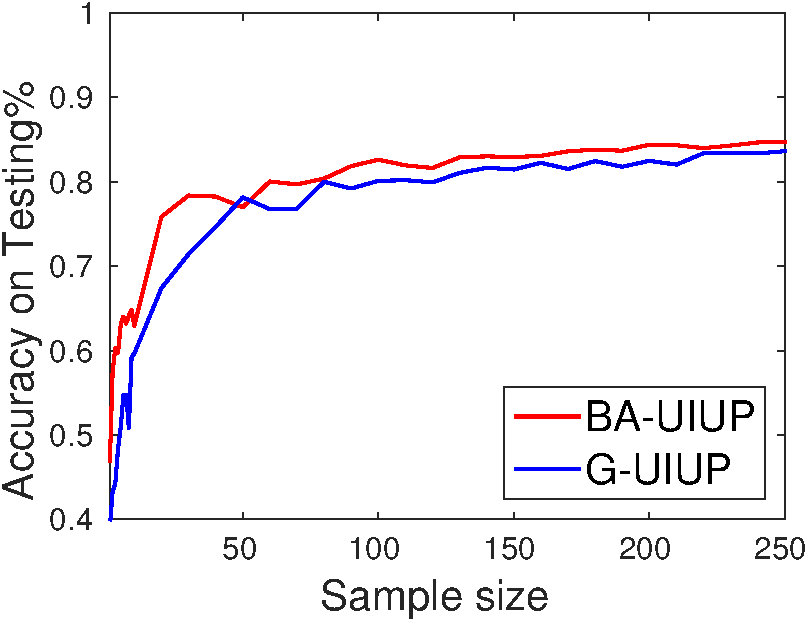
\includegraphics[width=0.95\textwidth]{figs/PrefLearnResults/Trees/CarEvaluation_Trees_X_MH.pdf}
			\captionsetup{font=scriptsize}
      \caption{CarEvaluation}
    \end{subfigure}
    \begin{subfigure}[b]{0.3\textwidth}
      \centering
      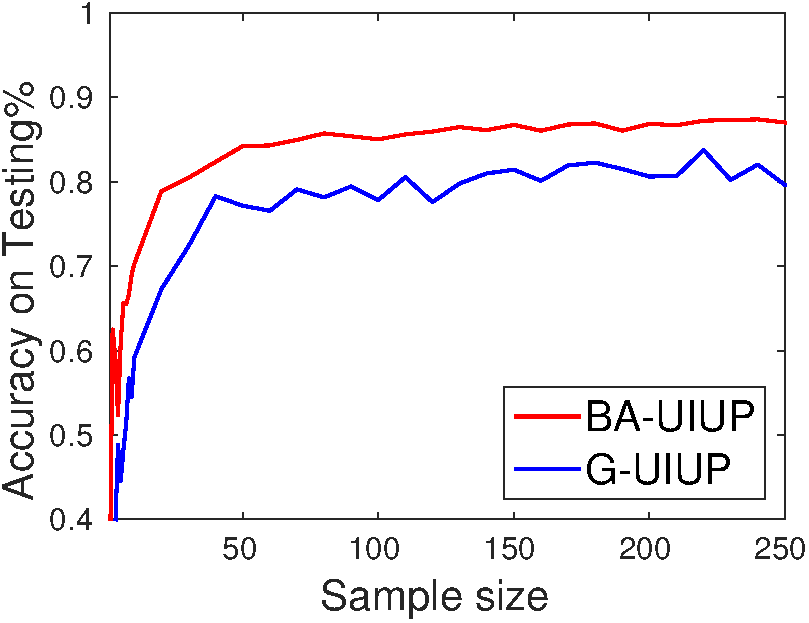
\includegraphics[width=0.95\textwidth]{figs/PrefLearnResults/Trees/IonosphereDownsampledFurther_Trees_X_MH.pdf}
			\captionsetup{font=scriptsize}
      \caption{Ionosphere}
    \end{subfigure}\\\vspace{0.3cm}
    \begin{subfigure}[b]{0.3\textwidth}
      \centering
      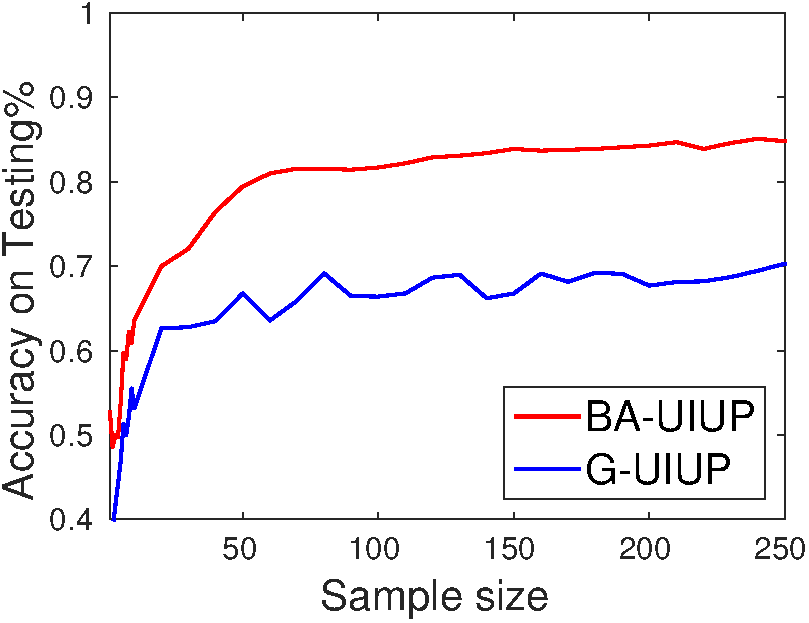
\includegraphics[width=0.95\textwidth]{figs/PrefLearnResults/Trees/MushroomDownsampled_Trees_X_MH.pdf}
			\captionsetup{font=scriptsize}
      \caption{Mushroom}
    \end{subfigure}
    \begin{subfigure}[b]{0.3\textwidth}
      \centering
      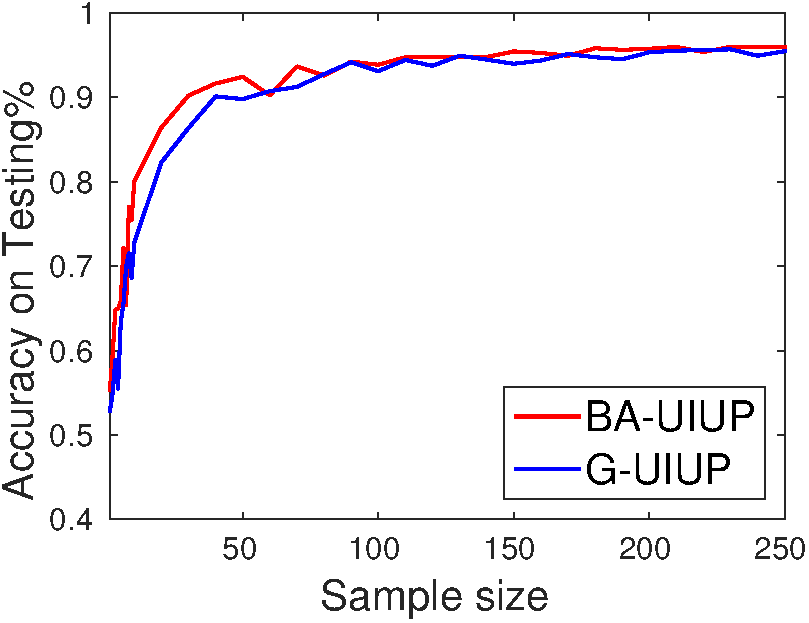
\includegraphics[width=0.95\textwidth]{figs/PrefLearnResults/Trees/WineDownsampled_Trees_X_MH.pdf}
			\captionsetup{font=scriptsize}
      \caption{Wine}
    \end{subfigure}

    \caption{Learning curves solving \tsc{MaxLearn} for UIUP PLP-trees}
  \end{figure}
}

\frameT{Experimental Results: Greedy}{
	\begin{table}
	  \centering
	  \small
		\setlength\tabcolsep{6pt}
	  %\begin{tabular}{ |c||c|c|r@{ | }l|c| }
	  \begin{tabular}{ |c||c|c|c|c| }
	    \hline
	    %Dataset          	 & UIUP & \multicolumn{2}{c|}{CIUP[D|B]}     & CICP \\
	    Dataset          	    & UIUP & CIUPB & CIUPD & CICP \\
	    \hline \hline                                    
	    BreastCancerWisconsin & 90.7 & 91.0  & 90.7  & \tbf{91.4}   \\ \hline
	    CarEvaluation         & 85.8 & 85.8  & 85.9  & \tbf{86.0}   \\ \hline
	    CreditApproval        & 91.4 & 91.6  & 92.0  & \tbf{92.2}   \\ \hline
	    GermanCredit          & 74.3 & 74.3  & 74.5  & \tbf{75.7}   \\ \hline
	    Ionosphere            & 87.1 & 87.2  & 88.5  & \tbf{90.4}   \\ \hline
	    MammographicMass      & 88.2 & 87.3  & 86.9  & \tbf{90.0}   \\ \hline
	    Mushroom              & 71.6 & 77.1  & 75.6  & \tbf{76.6}   \\ \hline
	    Nursery               & 92.9 & 93.0  & 93.0  & \tbf{93.0}   \\ \hline
	    SPECTHeart            & 93.4 & 95.4  & 94.8  & \tbf{95.7}   \\ \hline
	    TicTacToe             & 73.9 & 74.4  & 75.4  & \tbf{76.2}   \\ \hline
	    Vehicle               & 79.2 & 80.3  & 80.0  & \tbf{81.2}   \\ \hline
	    Wine                  & 95.5 & 97.8  & 97.5  & \tbf{97.8}   \\ \hline
	  \end{tabular}
	  \caption{Accuracy percents on the testing data (30\% of $\cE^\succ$)
						 for all four classes of PLP-trees, using models learned
						 by the greedy algorithm from the learning 
						 data (the other 70\% of $\cE^\succ$)}
	  \label{tbl:trees2}
	\end{table}
}

\frameT{Experimental Results: Sizes of PLP-trees by Greedy}{
	\begin{table}
	  \centering
		\small
		\setlength\tabcolsep{6pt}
	  \begin{tabular}{ |c||c|c|c| }
	    \hline
	    Dataset               & UIUP & CI       & $|\cE^{\succ}_{\train}|$ \\
	    \hline \hline                        
	    BreastCancerWisconsin & 9    & 87,381   & 6,306   \\ \hline
	    CarEvaluation         & 6    & 853      & 477,904 \\ \hline
	    CreditApproval        & 10   & 91,477   & 46,255  \\ \hline
	    GermanCredit          & 10   & 349,525  & 120,657 \\ \hline
	    Ionosphere            & 10   & 1,023    & 2,430   \\ \hline
	    MammographicMass      & 5    & 341      & 554     \\ \hline
	    Mushroom              & 10   & 91,477   & 5,913   \\ \hline
	    Nursery               & 8    & 7,765    & 383,644 \\ \hline
	    SPECTHeart            & 10   & 1,023    & 2,237   \\ \hline
	    TicTacToe             & 9    & 9,841    & 145,482 \\ \hline
	    Vehicle               & 10   & 349,525  & 53,699  \\ \hline
	    Wine                  & 10   & 349,525  & 7,225   \\ \hline
	  \end{tabular}
	  \caption{Maximum sizes of trees for all the classes and the 
						 training sample sizes for all datasets}
	  \label{tbl:trees_max_size}
	\end{table}
}

\frameT{Experimental Results: Sizes of PLP-trees by Greedy}{
	\begin{table}
	  \centering
		\small
		\setlength\tabcolsep{6pt}
	  %\begin{tabular}{ |c||c|c|r@{ | }l|c| }
	  \begin{tabular}{ |c||c|c|c|c| }
	    \hline
	    %Dataset          & UIUP & \multicolumn{2}{c|}{CIUP[D|B]}     & CICP \\
	    Dataset               & UIUP & CIUPB       & CIUPD  & CICP \\
	    \hline \hline                              
	    BreastCancerWisconsin & 6.7  & \tbf{19.8}  & 28.0   & 25.7    \\ \hline
	    CarEvaluation         & 6.0  & \tbf{73.2}  & 108.9  & 109.5   \\ \hline
	    CreditApproval        & 9.0  & \tbf{31.3}  & 78.6   & 81.1    \\ \hline
	    GermanCredit          & 9.7  & \tbf{49.8}  & 210.3  & 190.0   \\ \hline
	    Ionosphere            & 9.6  & \tbf{19.8}  & 31.5   & 30.6    \\ \hline
	    MammographicMass      & 4.5  & \tbf{8.3 }  & 10.8   & 10.0    \\ \hline
	    Mushroom              & 7.6  & \tbf{15.7}  & 22.7   & 16.3    \\ \hline
	    Nursery               & 8.0  & \tbf{56.2}  & 121.0  & 116.9   \\ \hline
	    SPECTHeart            & 8.4  & \tbf{13.0}  & 18.4   & 19.0    \\ \hline
	    TicTacToe             & 8.0  & \tbf{36.8}  & 126.8  & 115.2   \\ \hline
	    Vehicle               & 9.0  & \tbf{33.9}  & 101.3  & 105.4   \\ \hline
	    Wine                  & 5.1  & \tbf{14.2}  & 16.9   & 14.6    \\ \hline
	  \end{tabular}
	  \caption{Sizes of trees learned by the greedy algorithm from the training 
						 data (70\% of $\cE^\succ$)}
	  \label{tbl:trees_size}
	\end{table}
}

\frameT{Partial Lexicographic Preference Forests (PLP-Forests)}{
	\begin{enumerate}
		\item Inspired by \tit{random forests}, we proposed \tit{PLP-forests}
					that are sets of PLP-trees; thus, the four classes.
		\item To reduce the overfitting of a PLP-tree, a PLP-forest
		\begin{itemize}
			\item consists of \tit{diverse} trees (learned from \tit{small} training samples), and
			\item aggregates its constituent trees using the \tit{Pairwise Majority
						Rule} (PMR).
		\end{itemize}
	\end{enumerate}
}

\frameT{Experimental Results: Best-Agreement vs. Greedy}
{
	\begin{table}
	  \centering
		\small
	  \begin{tabular}{ |c||c|c| }
	    \hline
	    Dataset               & BA+UIUP              & G+UIUP \\
	    \hline \hline                     
	    BreastCancerWisconsin & \tbf{95.1}           & 93.4           \\ \hline
	    CarEvaluation         & 89.2                 & \tbf{91.9}     \\ \hline      
	    CreditApproval        & \tbf{93.1}           & 91.5           \\ \hline       
	    GermanCredit          & \tbf{77.9}           & 75.4           \\ \hline     
	    Ionosphere            & \tc{\tbf{92.5}}      & 83.0           \\ \hline   
	    MammographicMass      & \tbf{90.8}           & 89.1           \\ \hline         
	    Mushroom              & \tc{\tbf{90.2}}      & 78.8           \\ \hline 
	    Nursery               & \tbf{94.0}           & 93.2           \\ \hline
	    SPECTHeart            & \tbf{94.9}           & 93.7           \\ \hline   
	    TicTacToe             & \tbf{77.2}           & 75.1           \\ \hline 
	    Vehicle               & 81.9                 & \tbf{82.7}     \\ \hline
	    Wine                  & \tbf{96.9}           & 95.8           \\ \hline
	  \end{tabular}
	  \caption{Accuracy percents on the testing data (30\% of $\cE^\succ$)
						 for UIUP trees and forests of 5000 UIUP trees, 
						 using the greedy and the best-agreement algorithms from the learning 
						 data (the other 70\% of $\cE^\succ$)}
	  \label{tbl:forests1}
	\end{table}
}

\frameT{Experimental Results: Greedy}
{
	\begin{table}
	  \centering
		\small
	  %\begin{tabular}{ |c||c|c|r@{ | }l|c| }
	  \begin{tabular}{ |c||c|c|c|c| }
	    \hline
	    Dataset          			& UIUP & CIUPB & CICP \\
	    \hline \hline                             
	    BreastCancerWisconsin & 93.4 & 93.7  & \tbf{94.0} \\ \hline
	    CarEvaluation         & \tbf{91.9} & 91.4  & 91.4 \\ \hline
	    CreditApproval        & 91.5 & 92.8  & \tbf{93.0} \\ \hline 
	    GermanCredit          & 75.4 & 76.1  & \tbf{76.2} \\ \hline     
	    Ionosphere            & 83.0 & 89.3  & \tbf{89.5} \\ \hline   
	    MammographicMass      & 89.1 & 90.0  & \tbf{90.2} \\ \hline         
	    Mushroom              & 78.8 & \tbf{92.2}  & 91.8 \\ \hline 
	    Nursery               & 93.2 & 93.3  & \tbf{93.4} \\ \hline
	    SPECTHeart            & \tbf{93.7} & 93.6  & \tbf{93.7} \\ \hline   
	    TicTacToe             & 75.1 & 76.6  & \tbf{76.9} \\ \hline 
	    Vehicle               & 82.7 & 83.2  & \tbf{83.4} \\ \hline
	    Wine                  & 95.8 & 97.5  & \tbf{97.8} \\ \hline
	  \end{tabular}
	  \caption{Accuracy percents on the testing data (30\% of $\cE^\succ$)
						 for all four classes of PLP-forests of 5000 trees, 
						 using the greedy algorithm from the learning 
						 data (the other 70\% of $\cE^\succ$)}
	  \label{tbl:forests2}
	\end{table}
}

\frameT{Experimental Results: UIUP vs. CICP}
{
  \begin{figure}
    \centering
    \begin{subfigure}[b]{0.3\textwidth}
      \centering
      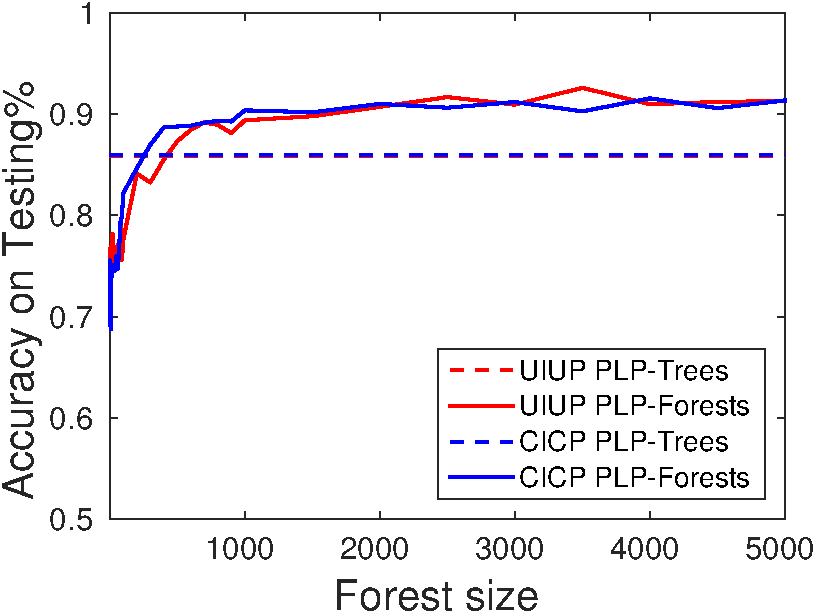
\includegraphics[width=0.95\textwidth]{figs/PrefLearnResults/Forests/CarEvaluation_Forests_MH.pdf}
			\captionsetup{font=scriptsize}
      \caption{CarEvaluation}
    \end{subfigure}
    \begin{subfigure}[b]{0.3\textwidth}
      \centering
      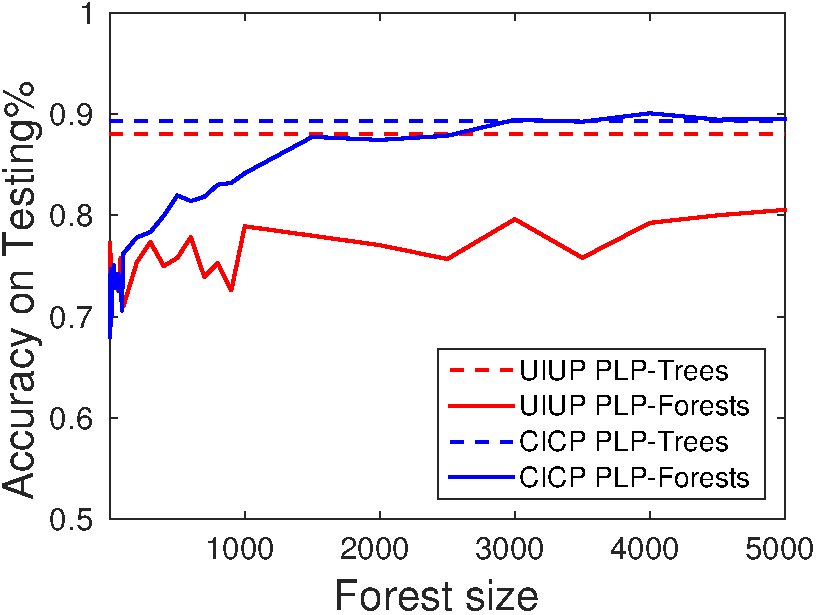
\includegraphics[width=0.95\textwidth]{figs/PrefLearnResults/Forests/IonosphereDownsampledFurther_Forests_MH.pdf}
			\captionsetup{font=scriptsize}
      \caption{Ionosphere}
    \end{subfigure}\\\vspace{0.3cm}
    \begin{subfigure}[b]{0.3\textwidth}
      \centering
      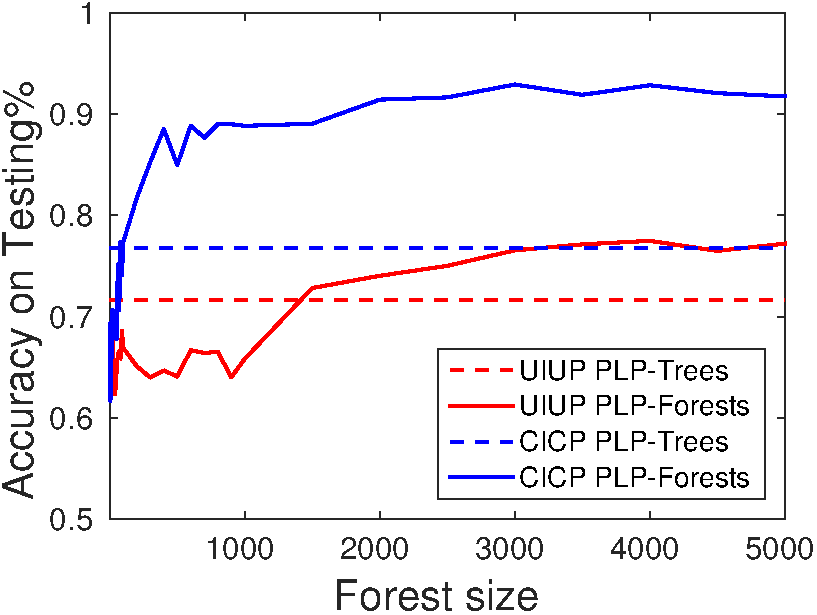
\includegraphics[width=0.95\textwidth]{figs/PrefLearnResults/Forests/MushroomDownsampled_Forests_MH.pdf}
			\captionsetup{font=scriptsize}
      \caption{Mushroom}
    \end{subfigure}
    \begin{subfigure}[b]{0.3\textwidth}
      \centering
      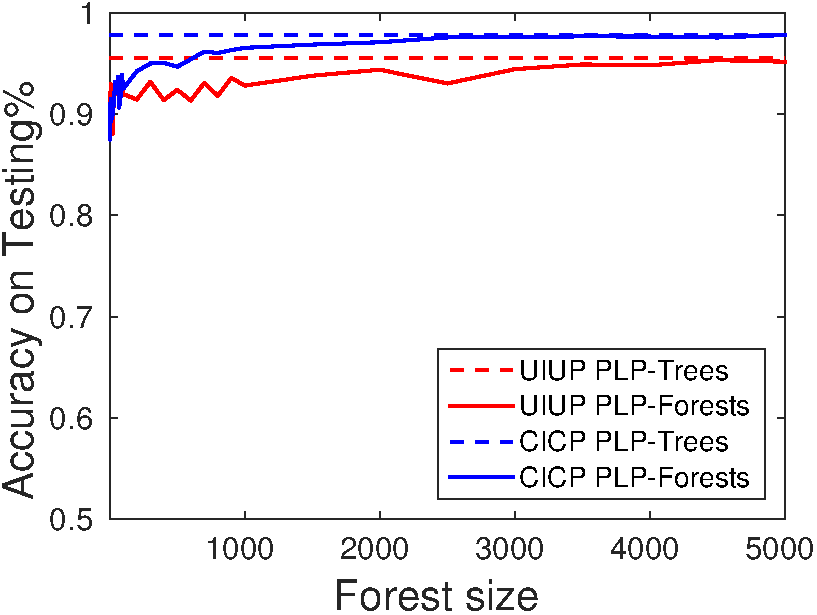
\includegraphics[width=0.95\textwidth]{figs/PrefLearnResults/Forests/WineDownsampled_Forests_MH.pdf}
			\captionsetup{font=scriptsize}
      \caption{Wine}
    \end{subfigure}

    \caption{Greedy learning curves solving \tsc{MaxLearn} for PLP-forests}
  \end{figure}
}

%\frameT{Preference Forests (P-Forests)}{
%	\begin{enumerate}
%		\item A \tit{preference forest} $F$ is a collection of PLP-trees
%					$F = \{T_1,\ldots,T_n\}$.
%		\item Denote by $N_F(o_1,o_2)=|\{T \in F:o_1 \succ_T o_2\}|$.
%		\item Given a preference forest $F$, and two outcomes $o_1$ and $o_2$, 
%					we say that $o_1 \succ_F^\Maj o_2$ iff $N_F(o_1,o_2)>N_F(o_2,o_1)$,
%					and that $o_1 \approx_F^\Maj o_2$ iff $N_F(o_1,o_2)=N_F(o_2,o_1)$.
%		\begin{itemize}
%			\item Pro: intuitive, decided in polynomial time.
%			\item Con: Condorcet paradox.
%			\item Other aggregating rules: positional scoring rules, Copeland's method, etc.
%		\end{itemize}
%	\end{enumerate}
%}
%
%\frameT{Experimental Results on P-Forests}{
%  \begin{figure}[ht!]
%    \centering
%      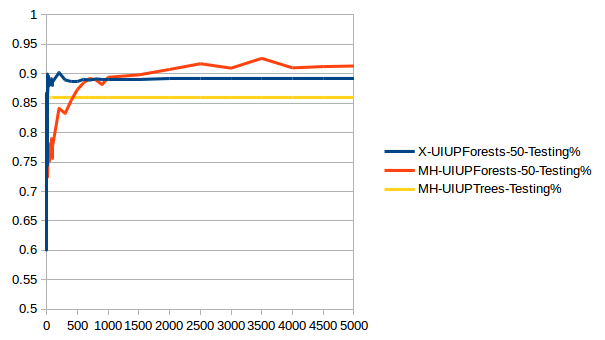
\includegraphics[width=0.7\textwidth]{figs/PrefLearnResults/Forests/X_MH/CarEvaluation.png}
%    \caption{Learning UIUP using ASP and greedy heuristic}
%  \end{figure}
%}
%
%\frameT{Experimental Results on P-Forests}{
%  \begin{figure}[ht!]
%    \centering
%      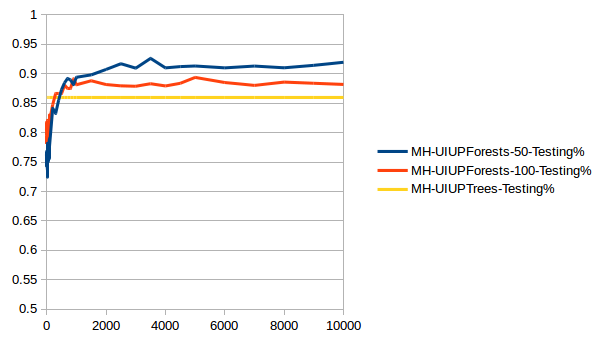
\includegraphics[width=0.7\textwidth]{figs/PrefLearnResults/Forests/MH/CarEvaluation.png}
%    \caption{Learning all four classes using greedy heuristic}
%  \end{figure}
%}

\frameT{Conclusion}{
	\begin{enumerate}
		\item PLP-trees and PLP-forests are \tit{expressive} preference models.
		\item PLP-forests aggregated by PRM provide in general \tit{higher} 
					accuracy than PLP-trees.
		\item PLP-trees and PLP-forests learned by a greedy approximation method 
					have accuracy \tit{comparable} to best-agreement PLP-trees and PLP-forests.
		\item The greedy algorithms are \tit{fast}, can work with \tit{large} 
					datasets (of $\sim$ half million examples), and can compute \tit{small}
					models.
	\end{enumerate}
}
